\chapter{State of the Art}
\label{sota}
\label{sec:secandtrust}

%%%%%%%%%%%%%%%%%%%%%%%%%%%%%%%%%%%%%%%%%%%%%%%%%%%%%%
%%%%%%        MODELLING SECURITY AND TRUST
%%%%%%%%%%%%%%%%%%%%%%%%%%%%%%%%%%%%%%%%%%%%%%%%%%%%%%
\begin{quote}
\textit{
In this chapter, we present the state of the art on \gls{voip} security research.
In Section~\ref{sota2012} we present the results of a survey reviewing 245 articles on \gls{voip} security and published in 2012 by Keromytis~\cite{keromytis2012comprehensive}.
As the first drafts of WebRTC specifications were published the same year, this survey is a solid starting point to understand the field of \gls{voip} security.
In Section~\ref{sec:sota2012+}, we present our own survey of \gls{voip} and WebRTC security research papers published between 2012 and 2017.
We follow a similar methodology as used by Keromytis and collect and classify 208 papers.
We then review the papers dealing specifically with WebRTC.
}
\end{quote}
\glsresetall
\section{VoIP Security Research - 2012}
\label{sota2012}
WebRTC is in 2018 still a young technology.
The \gls{w3c} WebRTC Working Group was created in May 2011 and the first version of the WebRTC Security Architecture draft was published in January 2012.
The same year, Keromytis published ``A Comprehensive Survey of Voice over IP Security Research''~\cite{keromytis2012comprehensive} which reviews 245 articles related to fields of \gls{voip} security.
This survey is a starting point for understanding the field of \gls{voip} security research just before the introduction of WebRTC. 
Indeed, WebRTC contributors built on the same accumulated experience when making design and implementation decisions.

In this section, we summarise Keromytis' survey and categorisation of \gls{voip} research topics.
We also give additional references from our personal knowledge when it seems relevant.
We particularly focus on research that could be applied in the context of WebRTC communication.
Note that a large part of the security research on \gls{voip} is focused on the network side such as the \gls{sip} signalling protocol and \gls{sip}-based architectures.
While WebRTC does not mandate a particular signalling architecture, \gls{sip}-based researches are still relevant to WebRTC.
Actually, \gls{sip} could be used on the signalling path, but more importantly, most vulnerabilities and defence mechanisms related to \gls{sip} are still relevant for ad-hoc signalling protocols.

\subsection{Threats Classification and Methodology}
\label{keromytis}
To build the survey, Keromytis initially collected papers from personal knowledge, searches on online library\footnote{CiteSeer, IEEE Xplore, ACM Digital Library, and Google Scholar.}, and browsing of proceedings of top security conferences, journals, and specific workshops\footnote{IEEE Security \& Privacy Symposium, ISOC Symposium on Network and Distributed Systems Security, ACM Computer and Communications Security, USENIX Security, RAID, ACM Transactions on Information and Systems Security, and IEEE Transactions on Dependable and Secure Computing.}.
In particular, searches were conducted with the following keywords: ``VoIP security'', ``VoIP vulnerabilities'', ``VoIP attacks'', ``SIP security'', ``SIP vulnerabilities'', and ``SIP attacks''.
The collection was then expanded by browsing the proceedings of conferences in which these papers appeared and searching for other VoIP security papers by the same authors.
The process was iterated over until no new papers were added to the collection.

These papers were then manually classified according to an extended version of the \gls{voipsa} threat taxonomy~\cite{zar2005voip}.
The considered \gls{voipsa} threat classes are the following: social threats, traffic attacks, denial of service, and service abuse.
In addition, eight additional classes were considered: overviews and surveys, field studies and system/protocol analysis, performance analysis, authentication protocols, architectures, middleboxes, intrusion detection, and miscellaneous. 
Figure~\ref{fig:keromytis} presents the repartition of surveyed papers in these classes.

\begin{figure}
\begin{center}
    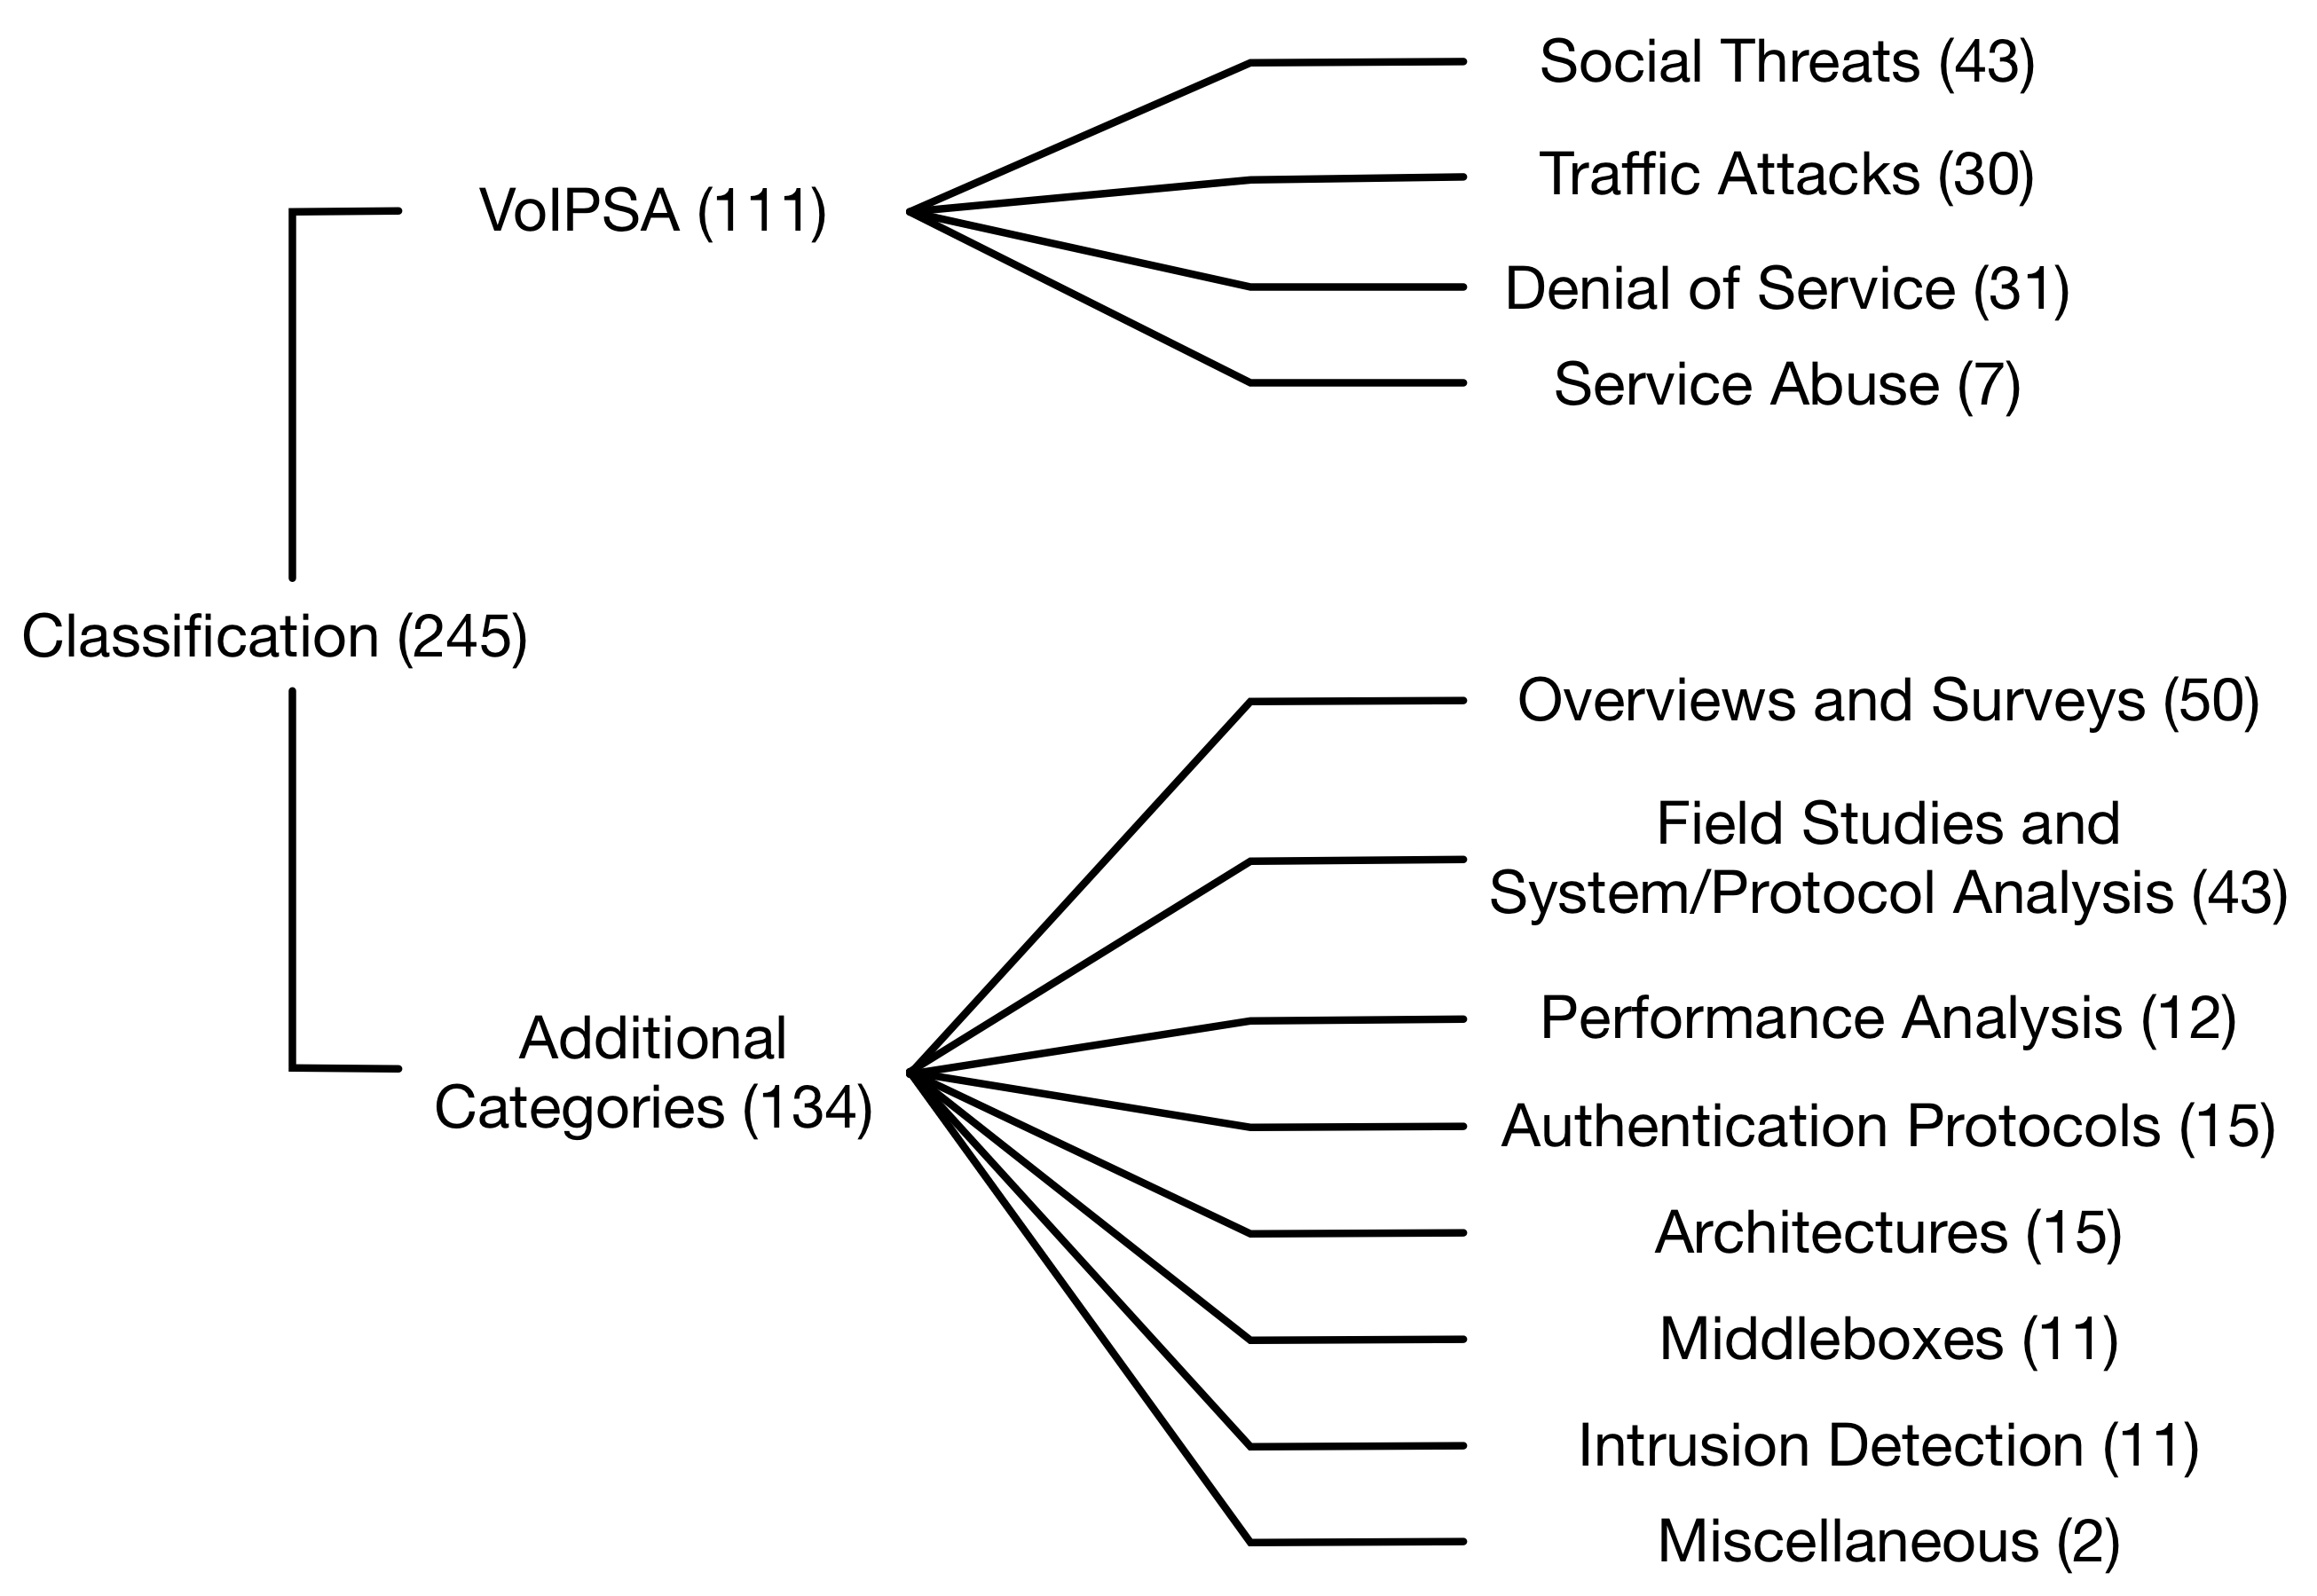
\includegraphics[scale=.5]{images/keromytis}
\end{center}
\caption{Classification tree~\cite{keromytis2012comprehensive}}
\label{fig:keromytis}
\end{figure}


\subsection{Keromytis Survey Summary}
\subsubsection{Social Threats}
Social Threats represent the attacks aimed at the human users rather than at the software systems.
Such attacks are for instance unwanted contacts misrepresenting the identity of a malicious calling party or bypassing opt-out consent.
In practice, research on social threats is mostly focused on defence against \gls{spit} call which we presented in Section~\ref{sec:availability}.

According to the \gls{voipsa}, the classification of call as spam is subjective. 
Indeed, \gls{spit} call may be lawful solicitations and become spam only after bypassing refused consent.
The bulk of defence against \gls{spit} thus focus on getting user's input.
Caller classification may follow a simple binary approach into whitelists or blacklists.
However, more complex approaches propose to use reputation-based models and social relations between users to assign a trust value to an incoming call.
In these systems, the intelligence of \gls{spit} detection algorithms is located at the endpoints and allow users to manage their own policies for \gls{spit} rejection.

Other approaches place \gls{spit} detection at the network level, \ie on the signalling path.
These systems measure various criteria such as the number of incoming and outgoing calls, call duration, and call history.
Deviation from standard long-term expected average may reveal a spam call.
These analyses may further be refined by user input or filtered with a Turing test\footnote{Turing tests tries to distinguish computers from humans.} presented to the caller.
Some authors also propose to apply fingerprinting techniques, either targeting \gls{sip} messages format or the audio data of incoming \gls{voip} calls.
\gls{spit} calls would be detected by the presence of unique fingerprint over a large number of different calls.
Sorge \etal\cite{DBLP:conf/icc/SorgeS09} propose to evaluate the reputation of \gls{cs} and their \gls{spit} detection algorithms, providing incentives to honest \gls{cs} to correctly tag outgoing calls.

Trust and reputation models may easily be bypassed under weak caller authentication.
Some authors thus propose to enforce strong caller identity verification.
In particular, Srivasta \etal\cite{srivastava2004preventing} propose to consider the caller origin domain and the confidence level in the authentication performed while Croft \etal\cite{croft2005model} propose to include a Verifying Authority into the call setup.
This Verifying Authority would be responsible for applying policies in particular based on the caller identity before transmitting the call to the user.

\subsubsection{Traffic Attacks}
The traffic attacks and defences class is concerned with the risks of eavesdropping, interception, and modification of signalling data and media sessions.
These attacks may either target unencrypted sessions or bypass cryptographically protected sessions.
This field of research, however, does not consider generic cryptography research but only focus on specific \gls{voip} cases.

Indeed, the specific nature of \gls{voip} traffic, transmitting voice in stream sessions, may allow specific attacks.
Some researchers thus propose to use packet delay variation (also referred to as jitter) in order to de-anonymise \gls{voip} streams or introduce covert channel.
Other researchers apply machine learning techniques to determine the language spoken or identify blank, phrases, or even words in encrypted voice streams.
As summarised in Figure~\ref{fig:vbrRecognition}, these attacks use packet size variation of \gls{vbr} human-speech codecs.
\gls{vbr} codecs, as opposed to Constant Bit Rate codecs, use variable packet size depending on factors such as encoded phonemes, blank in speech, or encoding quality.
As \gls{voip} is a time-sensitive application, delay or jitter may have a dramatic impact on the availability of the communication.
Thus reducing bandwidth usage and adapting to network conditions is a critical feature for \gls{voip} usability.
However, these researches reveal a trade-off between security and availability/quality of \gls{voip} communications.
\gls{rfc}~6562~\cite{RFC6562} gives guidelines on the usage of \gls{vbr} codecs in conjunctions with \gls{srtp} sessions.

\begin{figure}
\begin{center}
    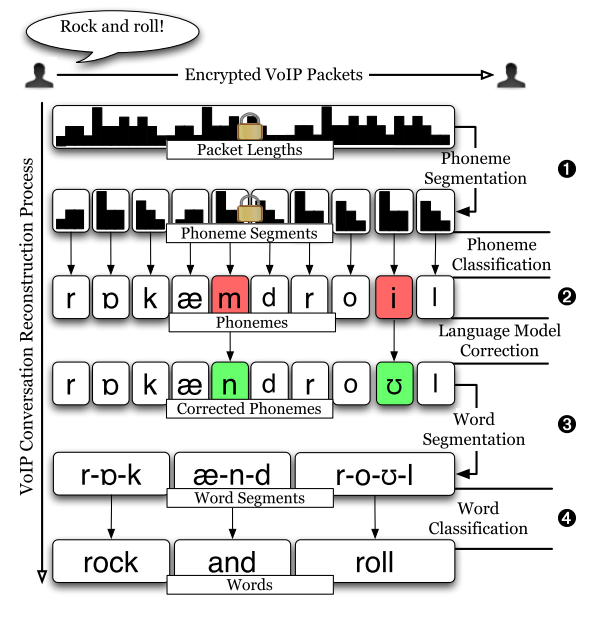
\includegraphics[scale=.5]{images/vbrRecognition}
\end{center}
\caption[VBR Transcripts Reconstruction]{Overall architecture of an approach for reconstructing transcripts of \gls{voip} conversations from sequences of encrypted packet sizes~\cite{White2011}.}
\label{fig:vbrRecognition}
\end{figure}

Traffic analysis and signalling data can be used to compromise users' privacy.
Some researchers study approaches based on anonymisation networks such as Tor (see Section~\ref{sec:tor}) and traffic padding techniques~\cite{DBLP:conf/acsac/MelchorDI07,DBLP:conf/cms/ZhangF10, }. 
Srivasta~\etal\cite{DBLP:conf/sp/SrivatsaLI08} study the issue of \gls{qos}-sensitive routes in anonymising networks. 
To this day, QoS is still an issue for \gls{voip} over anonymisation networks and researchers are still exploring possible solutions~\cite{DBLP:journals/popets/HeuserRPCDEKST17}.

A number of researches suppose unencrypted signalling paths or media session or focus on alternative key agreement protocols such as ZRTP. 
As WebRTC mandates the use of \gls{dtls} and \gls{srtp} for media and data sessions, and browsers enforce the use of \gls{tls} for signalling session, we do not consider these results as relevant to our research.

\subsubsection{Denial of Service}
We presented \gls{dos} attacks in Section~\ref{sec:availability}.
While \gls{dos} attacks may target either endpoints or networks elements, researches in this field mostly focus on attack and detection at the network level.
\gls{dos} flooding attacks, schematised in Figure~\ref{fig:dos}, have similarities to \gls{spit} calls meaning that these can be detected by monitoring deviation from standard call frequencies or error rate. 
Legitimate situations such as emergencies may also conduct to flooding scenarios.
Some researchers thus try to differentiate \gls{dos} attacks from flash crowds situations~\cite{DBLP:conf/ccs/FuchsALM08}.
However, the main difference with \gls{spit} is that \gls{dos} attacks aim at shutting down the \gls{voip} network.
It is crucial for detection algorithms to introduce as few overheads as possible during call setup.

Indeed, other \gls{dos} attacks directly aim at flooding the memory or CPU of network elements and in particular \gls{sip} servers.
While strong message authentication is proposed as a solution against \gls{dos} attacks, some researchers show that authentication may have a negative impact in some \gls{dos} scenarios~\cite{DBLP:conf/noms/LuoPL08}. 
Whitelisting or lightweight authentication based on call history from regular caller's identity or \gls{ip} adress, actually similar to some trust models, are proposed to mitigate attacks.
Other mitigation techniques also propose to adapt server procedures during \gls{dos} scenarios, for instance, dropping ringing call earlier when being overloaded~\cite{DBLP:conf/ism/ConnerN08}.

\begin{figure}
\begin{center}
    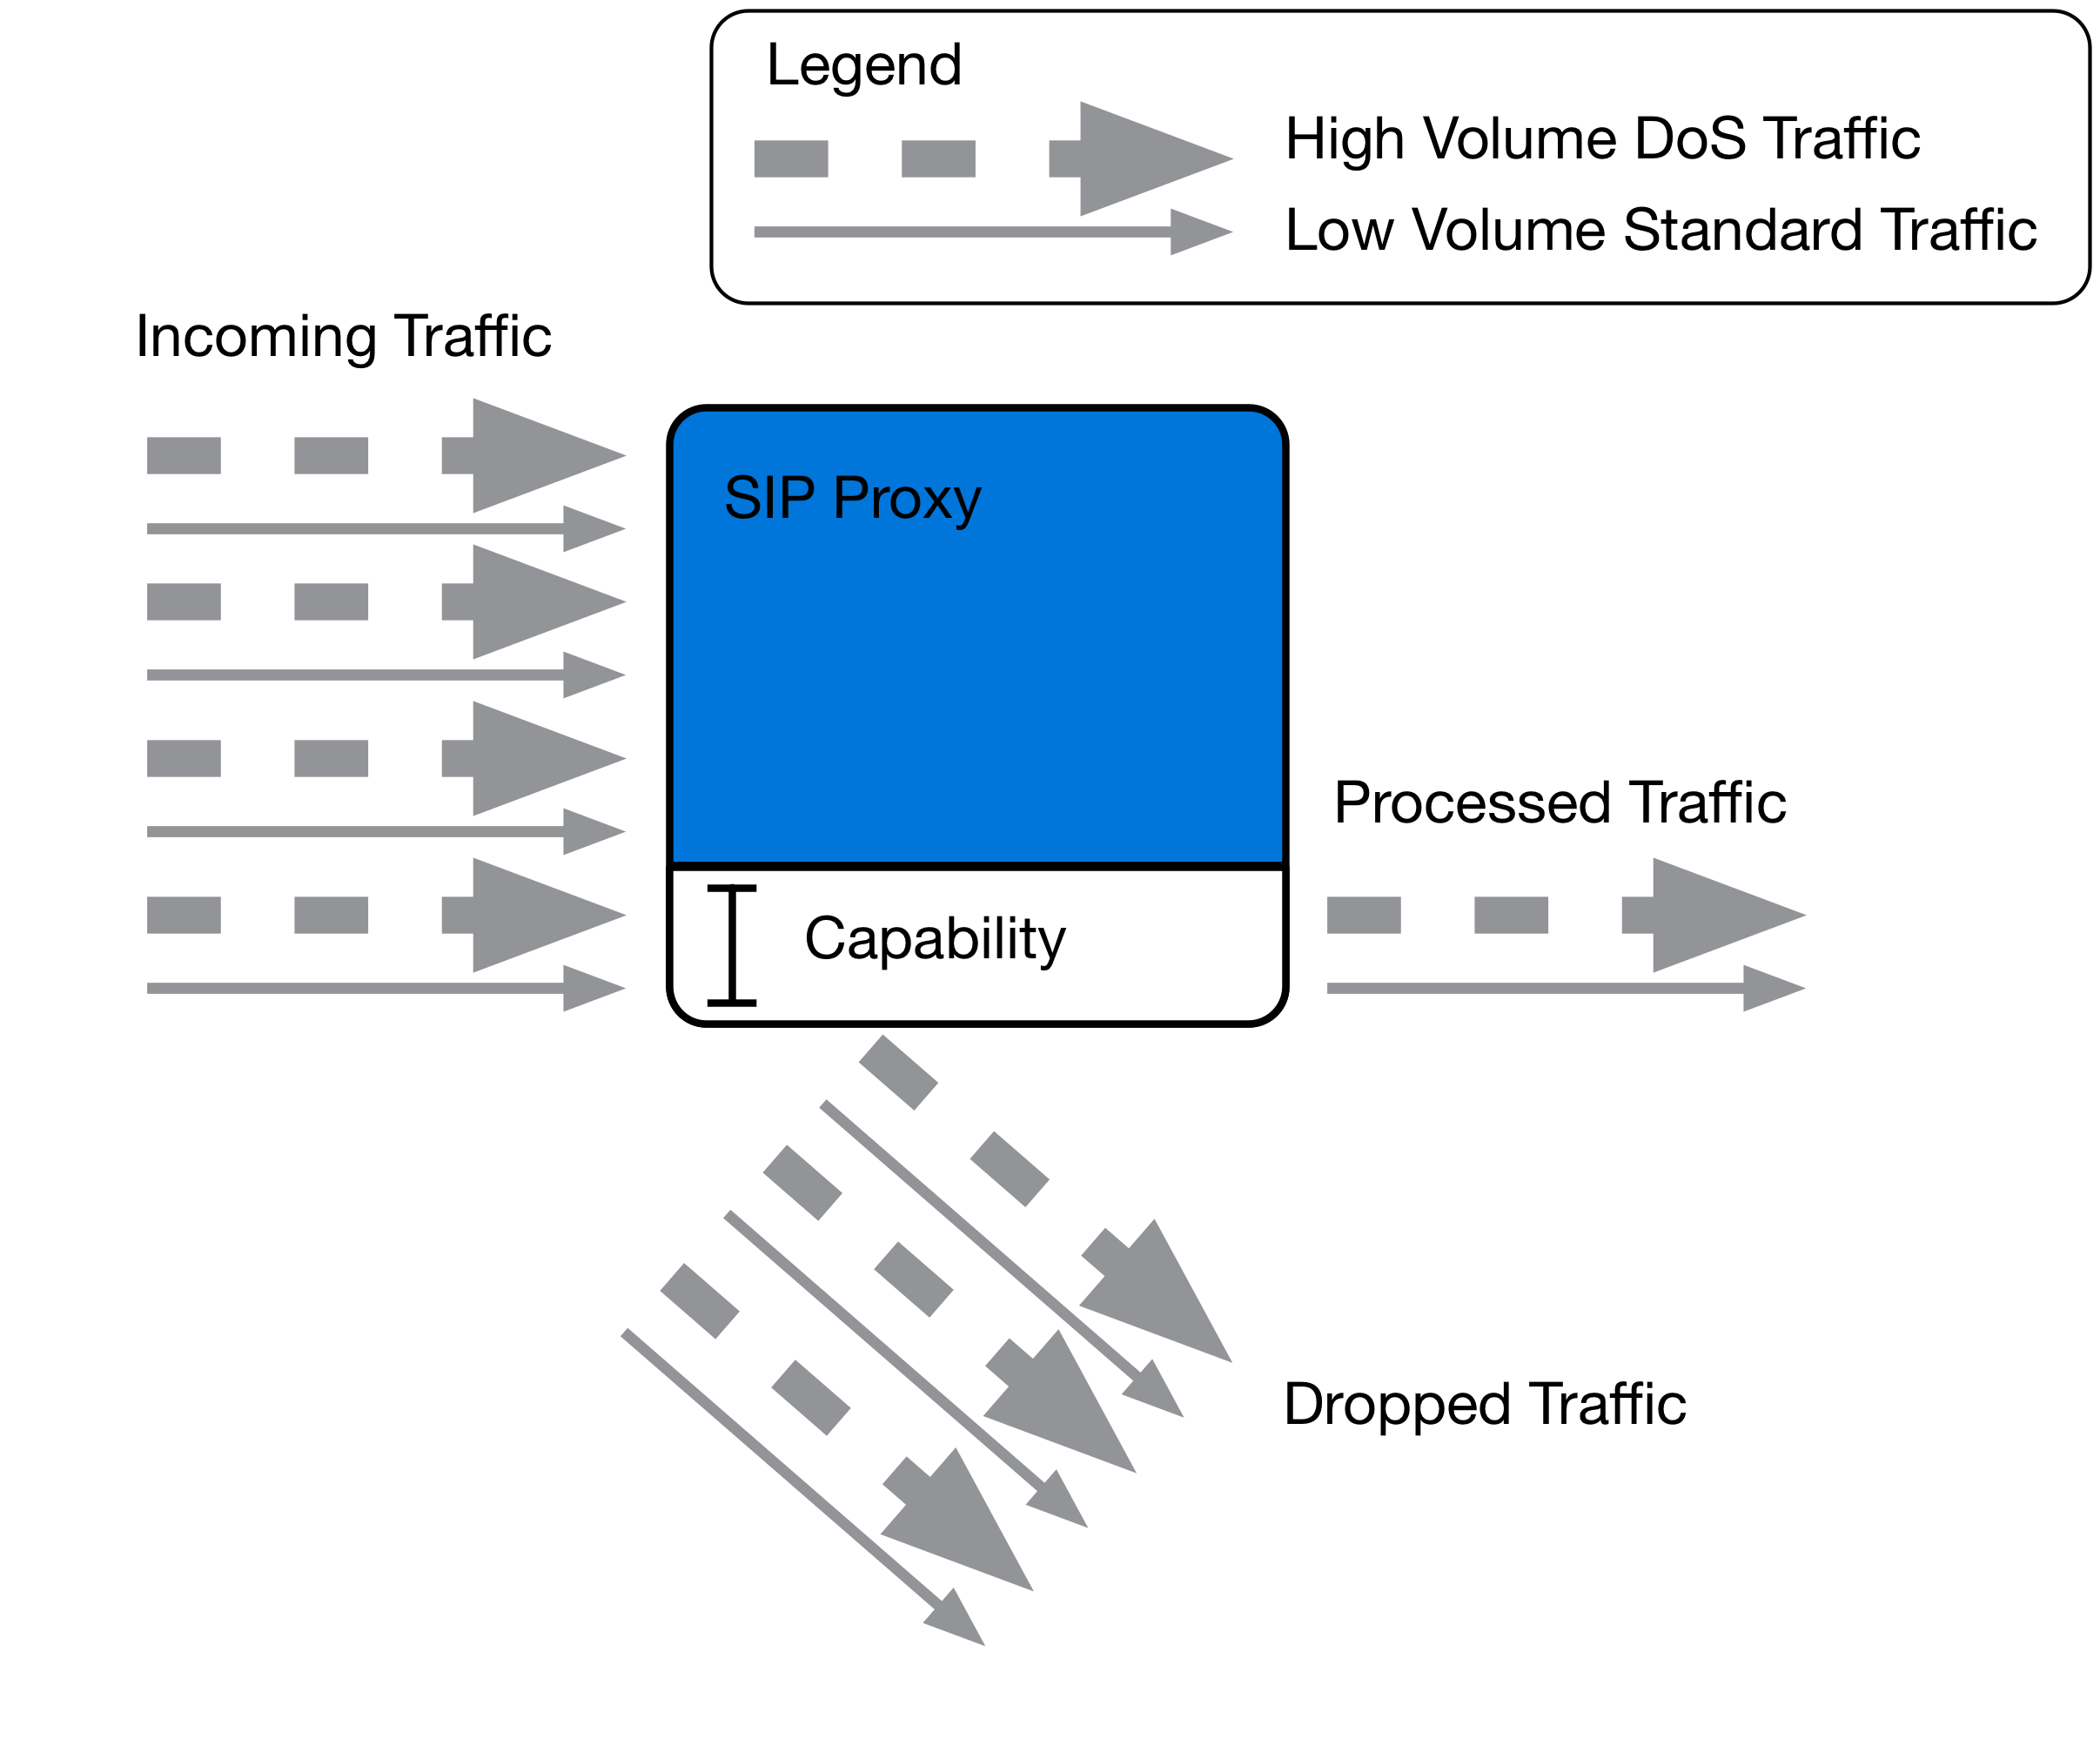
\includegraphics[scale=.5]{images/dos}
\end{center}
\caption[Denial of Service Flooding Attack]{Schematic overview of a \gls{dos} flooding attack. Due to the server's limited processing capabilities a lot of regular requests cannot be processed if a high load of malicious messages are targeted towards the server~\cite{ehlert2010survey}.}
\label{fig:dos}
\end{figure}

Payload and flow tampering attacks target specific signalling protocols, respectively to crash servers or abort sessions.
Most research on these attacks focus on \gls{sip} and protection mechanisms are well-known~\cite{ehlert2010survey} including tools to check \gls{sip} implementations.
Additionally, encryption on the signalling path deters flow tampering attacks.


\subsubsection{Service Abuse}
Service abuse threats are related to the improper use of \gls{voip} services especially in commercial services, for instance, to increase or avoid billing.
The research in this area is quite limited compared to other threat classes as it features only 7 references.
This can be explained by the specificity of architectures concerned by service abuse threats.
Billing is closely associated with authentication and authorization of users.
Some described attacks use a \gls{sip} protocol vulnerabilities revealed by formal verification to forge \gls{sip} messages impersonating users.
A solution to fraud and proposed by Geneiatakis \etal\cite{geneiatakis2008mechanism} is to let an \gls{aaa} server sign \gls{sip} messages after the user authenticated to the server, hence providing authenticity and non-repudiation for signalling messages. 
Although the solution is based on Telco rather than web protocols, it shows similarity to the introduction of a third-party \gls{idp} in WebRTC communication setup.


\subsubsection{Field Studies and System/Protocol Analysis}
Researches in this category focus on analysing protocols, implementations, and deployed systems using various techniques in order to find security vulnerabilities and flaws. 
Techniques used include formal verification~\cite{DBLP:conf/csfw/GuptaS07}, fuzzy testing~\cite{DBLP:conf/im/AbdelnurSCP07}, as well as black-box~\cite{DBLP:conf/infocom/BasetS06} or source code analysis~\cite{berson2005skype}. 
Similar analyses are also conducted in paper classified in other categories.

Formal verification techniques ensure that supposing a defined attacker model, the attacker cannot learn compromising information.
Such an attacker model is the Dolev-Yao~\cite{dolev1983security} model in which the attacker can listen to any message on the network, build arbitrary messages from known information, and send them over to the network.
The AVISPA project\footnote{\url{avispa-project.org}}, for Automated Validation of Internet Security Protocols and Applications, is a suite of tools for formal modelling and verification of security protocols.
In particular, the project offers a library of protocol models in the High-Level Protocol Specification Language, some with known and demonstrated attacks.

Formal verification should not hide the fact that actual implementations may present faults and weaknesses. 
These faults may be due to weak specification, error in the implementation, or use of default configurations.
For instance the Heartbleed bug\footnote{\url{heartbleed.com}} allowed an attacker to reveal the memory of an OpenSSL protected system, the most popular \gls{tls} implementation, by using a missing bound-check in the handling of the \gls{tls} heartbeat\footnote{The actual fix shows how a small implementation error can have dramatic consequences: \url{https://git.openssl.org/gitweb/?p=openssl.git;a=commitdiff;h=96db902}}.

A number of surveyed work resulted in vulnerability disclosure publications in databases such as the \gls{cve} database.
Such database allows the rapid dissemination of vulnerability disclosures and fixes to organisations using security software.


\subsubsection{Performance Analysis}
Performance analysis works focus on evaluating the impact of security protocols on both call setup and media sessions.
We already mentioned the trade-offs between security and availability/quality of the communications.
Papers in this category try to precisely measure this trade-off.

Results globally show that the main overhead is due to the asymmetric encryption of signalling messages while the symmetric encryption of the media session only produces a small overhead.
The exact figures vary depending on the actual protocol and configurations being compared.
For instance, a prototype demonstrates an improvement from a factor between 2 and 8 in handled call setup requests per second by using the Elliptic Curve DSA algorithm instead of RSA.

Other researches, not referenced in the survey, evaluate the strength of cryptographic protocols.
In practice, perfect security is highly impracticable and only imperfect security can be achieved~\cite{Shannon1949}.
Modern cryptography thus aims for a high enough security given reasonable computation power. 
Guessing attacks (or brute-force) form an upper-bound to the amount of computation required to break an encryption.
Against some encryption schemes, faster techniques than exhaustive search can be used.
To estimate the difficulty of an attack against these encryptions it is necessary to factor computation time and cost in the equation. 
For instance, Kleinjung et al.~\cite{Kleinjung2012} use Amazon cloud public prices to compare the security level of current algorithms with the level of the DES in 1980, as proposed by Lenstra~\cite{Lenstra2004}. 
As the computing power increases and computing cost decreases over time these estimations must be updated regularly. 
National security agencies~\cite{ANSSI, NIST} also give recommendations on security algorithm implementations and usages to achieve reasonable security properties in a given timeframe.

Alia \etal\cite{alia2010putting} propose a component-based adaptation model to manage the trade-offs between \gls{qos} and Security.
They model the adaptable \gls{voip} system as a composition of components each providing different \gls{qos} and security properties.
A utility function aggregating \gls{qos} and security dimensions, shown in Figure~\ref{fig:utilityFunction}, allows discriminating between different configurations.
Considered dimensions are the latency and video scheme quality for \gls{qos} and the confidentiality, anonymity, and authentication for security.
Their model also uses user's preferences as weight in the utility function and risk context as minimal required value for each security dimensions.

\begin{figure}[H]
\begin{center}
$U = W^{lat}.F(lat) +  W^{qua}.F(qua) + W^{conf}.F(conf) +$\\

$ W^{anon}.F(anon) + W^{auth}.F(auth)$
\end{center}
\caption[Alia~\etal\cite{alia2010putting} Utility Function]{Overall utility function~\cite{alia2010putting} with $F(k)$ the utility functions and $W^k$ the user preference weights for dimensions $k$ as latency, video scheme quality, confidentiality, anonymity, and authentication.}
\label{fig:utilityFunction}
\end{figure}

\subsubsection{Authentication Protocols}
The \gls{sip} authentication mechanism is based on \gls{http} digest authentication~\cite{RFC3261} and allows any \gls{sip} proxy or \gls{sip} user-agent to issue an authentication challenge when receiving a request. 
The response to the challenge is basically a hash of some information including a nonce, \ie a unique random number associated with the request, and a password.
The response also includes a username.
Upon receiving the response, the entity which issued the challenge looks up the password corresponding to the submitted username. 
It can then perform the same digest operation and compare the result to the given digest response to validate it.

Researchers working on authentication protocols mainly propose extensions or variants to \gls{sip} authentication and are mostly focused on \gls{voip} as a use case for cryptography.
Interestingly, an article published by Cao and Jennings~\cite{cao2006providing} in 2006 deals with the issue of end-to-end user identity in \gls{voip} call establishment.
One of their assumptions is that using TLS over each signalling hop is unrealistic\footnote{The authors explains this as to be ``because of some difficulties and other reasons for deploying TLS''~\cite{cao2006providing}.}, thus breaking the necessary chain of trust.
In 2017 this assumption cannot be considered valid anymore and the WebRTC security architecture recommends for the signalling path to be secured by TLS\footnote{``[The signalling] message is sent to the signalling server, e.g., by XMLHttpRequest or by WebSockets preferably over TLS''~\cite{I-D.ietf-rtcweb-security-arch}.}.


\subsubsection{Other categories}
Other research surveyed by Keromytis are categorised as middleboxes, architectures, and intrusion detection aiming at various threats but ``not easily classified in any of the previous categories''.
Middleboxes are network devices manipulating traffic for other purposes than packet forwarding.
Researches on \gls{voip} middleboxes thus focus on the traversal and operation of firewall and gateways to other networks.
Architecture and intrusion detection researches mainly focus on the detection of anomalies in \gls{voip} networks, either from malicious or non-adversarial causes and related defences.


\subsubsection{Observations}
According to Keromytis observations, almost 20\% of the surveyed publications offer an overview of \gls{voip} security problems and solutions.
He also observes that over 15\% of the work is coming from the cryptographic community, either to increase security or performance and that roughly 20\% of researches are dedicated to addressing \gls{spit}.
While he remarks that \gls{spit} is not currently an issue for \gls{voip}, he adds that prior and current experiences in email and telemarketing spams should be sufficient motivations to continue researches against \gls{spit}.

Comparatively, he observes that the problem of \gls{dos} is less studied and that researches on the subject focus on the network side of things. 
In previous surveys on the \gls{cve} database, Keromytis reported a majority of \gls{sip}-specific \gls{dos} vulnerabilities with half of the \gls{dos} vulnerabilities present at the endpoint.
He thus argues for more research targeting this problem, especially looking at strengthening implementations and not addressing the problem from a black-box approach.
Finally, Keromytis also argue for more work addressing cross-protocol and cross-implementation problems.


\section{VoIP and WebRTC Security Research - 2012+}
\label{sec:sota2012+}
\label{sec:vapen}
To complete our state of the art we survey and categorise \gls{voip} research and published since 2012.
We first present our methodology for collecting papers.
We then give a rough overview of the repartition of \gls{voip} research since 2012 by classifying collected papers.
Finally, we review collected papers dealing specifically with WebRTC.

\subsection{Methodology}
To build our survey we first look at collecting papers related to \gls{voip} security research and published between 2012 and 2017.
We use the same keywords as Keromytis~\cite{keromytis2012comprehensive}, that is: ``VoIP security'', ``VoIP vulnerabilities'', ``VoIP attacks'', ``SIP security'', ``SIP vulnerabilities'', and ``SIP attacks''. 
As WebRTC was introduced in 2012 and is the focus of our research, we also look for papers specifically targeting WebRTC.
To this end we use WebRTC as an additional keywords, \ie ``WebRTC security'', ``WebRTC vulnerabilities'', ``WebRTC attacks''.
The search is finally conducted on Google Scholars search engine and using the search strings presented in Figure~\ref{fig:searchString}.

\begin{figure}[H]
\begin{center}
``VoIP OR SIP OR WebRTC Security OR Vulnerabilities OR Attacks ''\\

``WebRTC Security OR Vulnerabilities OR Attacks ''
\end{center}
\caption{Paper collection search strings used on Scholar.}
\label{fig:searchString}
\end{figure}

Google Scholar indicates 27 800 results for the first search string and 2 890 results for the second string.
We crawl these results, ordered by relevance until we estimate that proposed papers are not relevant anymore.
Paper selection is done based on title and abstract, and ultimately our paper collection on \gls{voip} research returns 208 results.
We do not consider non-peer reviewed papers. Relevant \gls{rfc} are presented in the background Chapter~\ref{security} on WebRTC trust and security architecture. 

\subsection{Observations on VoIP Security Research since 2012}

\begin{table}
\begin{tabular}{{@{}lcccc@{}}}\toprule\toprule
  \textbf{Category} & \textbf{-/2012} & \textbf{2012/2017} & \textbf{diff} & \textbf{WebRTC} \\\midrule
  \textbf{Denial of Service} & $12.6\%$ (31) & $16.4\%$ (33) &  $+ 3.8\%$ & $0$ \\
  \textbf{Service Abuse} &$  2.9\%$ (7) &$ 5\%$ (10) &$ + 2.1\% $& 0\\
  \textbf{Social Threats} &$ 17.5\%$ (43) &$ 6.5\%$ (13) &$ - 11\% $& 1 \\
  \textbf{Traffic Attacks} &$ 12.2\%$ (30) &$ 5\%$ (10) &$ - 7.3\% $& 2 \\\midrule
  \textbf{Overviews and Surveys} &$ 20.4\%$ (50) &$ 15.9\%$ (30) &$ - 4.5\% $& 7 \\
  \pbox{20cm}{\textbf{Field Studies and} \\ \textbf{System/Protocol Analysis}} &$ 4.9\%$ (12) &$ 8.9\%$ (18) &$ + 4\% $& 2 \\
  \textbf{Performance Analysis} &$ 5.7\%$ (14) &$ 7.5\%$ (15) &$ + 1.8\% $& 0 \\
  \textbf{Authentication Protocols} &$ 6.1\%$ (15) &$ 16.4\%$ (33) &$ + 10.3\% $& 1 \\
  \textbf{Architectures} &$ 7.7\%$ (19) &$ 10.4\%$ (21) &$ + 2.7\% $& 8 \\
  \textbf{Middleboxes} &$ 4.5\%$ (11) &$ 1\%$ (2) &$  - 3.5\% $& 2\\
  \textbf{Intrusion Detection} &$ 4.5\%$ (11) &$ 4.5\%$ (9) &$ - $& 0\\
  \textbf{Miscellaneous} &$ 0.8\%$ (2) &$ 2.5\%$ (5) &$ + 1.7\% $& 0 \\\midrule
  \textbf{Total} & 100\% (245) & 100\% (201) & & 23\\\bottomrule
  \hline
\end{tabular}
\caption{Classification of VoIP security papers returned by our search.}
\label{tab:classificationPaper}
\end{table}

We roughly classify our collection of 208 papers, based on title and abstract, into the same categories as presented in Section~\ref{keromytis}.
This allows to compare the proportion of results for both periods and get a picture of the repartition of researches.
Table~\ref{tab:classificationPaper} shows the classification of collected papers and compare them with the repartition of paper collected by Keromytis.

According to our classification, we observe some significant changes ($> +/-5\%$) in the repartition of research.
Firstly, we observe a drop in the proportion of research focusing on social threats by $11\%$ for the period since 2012. 
Keromytis remarked that most of the social threat researches were focused on \gls{spit} mitigation, although it was not an issue in \gls{voip} yet. 
This fact may explain the decrease in research for this threat category.
Researches focused on traffic attack also decreased by more than $7\%$ on the same period.
In particular, we do not observe any research related to traffic attack since 2016 and we classify only one 2015 paper as traffic attack related.
Conversely, the authentication protocol category of research sees an increase of more than $10\%$.
In particular, we collected multiple papers applying elliptic-curve cryptography to \gls{voip} while in Keromytis's survey only two references are given.
Note that some of these differences may be due to the way we collected and classified papers compared to Keromytis process.

We then looked for references to WebRTC in surveyed papers.
We extracted a list of authors of these WebRTC security papers and looked for any missing publications using DBLP\footnote{\url{dblp.uni-trier.de}}, revealing two additional overview papers.
Unsurprisingly, the categories of Denial of Service, Service Abuse, and Intrusion Detection do not contain WebRTC related research.
Such attacks are generally targeted against the service architecture which is not the focus of the WebRTC specification.
Similarly, the social threats and traffic attacks categories only contain one and two WebRTC related paper respectively.
While WebRTC mandates or recommends the use of some security mechanisms on the signalling and media paths security, researches in these areas are not specific to WebRTC and may target out-of-scope protocols such as \gls{sip}.
Surprisingly, although WebRTC does not specify any signalling architecture we observe several WebRTC papers in the architecture and middleboxes categories.
A large proportion of these papers are dealing with issue of integrating WebRTC services inside enterprise environment and existing \gls{voip} infrastructures.

\subsection{Survey of WebRTC Security Research}

\subsubsection{Traffic Attacks (2)}
In their 2015 articles, Mauro and Longo~\cite{di2015decision,mauro_revealing_2017} use machine learning techniques to identify encrypted WebRTC traffic.
Used classifier algorithms are configured to consider the inter-arrival times, packet lengths, and the number of packets received and sent.
They implemented a detection system and tested it with three then four classification algorithms.
Their results are however limited in significance due to the small and artificial test sample.

%Burgstaller \etal propose to build an onion routing layer on top of WebRTC in order to provide anonymity to participants. Their architecture relies on a protocol stack organised in three layers (see Figure~\ref{}). 
%The peer-to-peer communication layer manages individual connections between nodes and is built using WebRTC.
%The onion layer routes packets inside an onion chain, web workers are used to decrypt the onion layers.
%Finally, an end-to-end communication layer allows to securely route message between two onion chains.
%An implementation is referenced
% --> Use WebRTC but does not provide anonymity to WebRTC

\subsubsection{Overviews and Surveys (6)}
In 2013, one year after the first WebRTC drafts, Jennings \etal\cite{jennings2013real} published an overview of the WebRTC architecture and its design principle.
They present the security and identity architecture, in particular, mentioning that their approach aims at allowing users to ``use their preferred identity provider and logs on to the provider in whatever way that provider uses''.
A similar overview paper is published in 2014 by Barnes and Thomson~\cite{barnes2014browser} this time focusing on the security and identity architecture exclusively.

Loreto and Romano published in 2012~\cite{loreto_real-time_2012} an overview of the ongoing efforts for WebRTC specifications in which they discuss some security considerations.
In July 2017 they published an overview of the remaining efforts towards WebRTC~1.0~\cite{loreto_how_2017}.

Rahaman published an overview on WebRTC security in 2015~\cite{rahaman2015survey}.
After presenting the WebRTC security architecture, examples of trusted third-parties \gls{idp} are provided: Google, Facebook, LinkedIn, as well as the Browser Id and WebFinger protocols.
Rahaman also lists concerns for WebRTC security including the inheritance of \gls{voip} attacks through gateways and the security of third-party \gls{idp}. 
No details are however given on particular attacks. 
Issues of gateway implementation to integrate WebRTC service with \gls{sip}-based systems are also the subject of a 2013 paper by Amirante \etal\cite{amirante2013seamless}.
%
%Feher \etal published an overview of WebRTC security threats associated with particular WebRTC clients. 
%The threats considered are server crashes due to malformed JSON and server takeover, JavaScript injection attacks in web client, malware in android clients, and traffic eavesdropping. 
%They also reference mitigation techniques for some threats.
%\todo{Feher works seems to not be peer-reviewed -no reference to conference or journal, nor on Scholar or Dblp ...}

The Strategic Research Roadmap for European Web Security project's (STREWS)\footnote{The STREWS project was a European research project running between 2012 and 2015.} major contribution is a technical state of practice document for web security~\cite{de2013web}.
The project's studied methodology targets new aspects added to the web ecosystem in parallel with the standardisation and deployment of the technology bringing these aspects.  
Following this methodology, the project published a security case study report on WebRTC~\cite{bos2014case} as it was deemed a ``security sensitive extension to the Web''.
This document identifies six assets related to WebRTC and describes new threats.
These assets are the browser, the client machine, the server machine, the client-side application code, the identity provider's infrastructure, and \gls{stun}/\gls{turn} servers.
The threats described cover a large scope including some \gls{dos} attacks, service abuse attacks, \gls{mitm} attacks, and privacy attacks.
In the second part of the document, a few areas are studied in-depth and new attacks and vulnerabilities are described including:
\begin{itemize}
\item In additions to \gls{mitm} attacks, malicious web applications can also redirect both streams to an attacker either by accessing streams directly from JavaScript or by taking screenshots using the HTML canvas elements containing the video streams.
\item The central position of \gls{idp} means that they can be used as a meta-data capture service, for instance, to allow legal pervasive monitoring or user profiling.
\item The WebRTC identity architecture allows the disclosure of precise user identity information to malicious web applications.
\item The web certificate infrastructure does not have an effective scoping of \gls{ca}'s authority. This issue extends to \gls{idp} handling caller authentication in many WebRTC scenarios.
\end{itemize}

\subsubsection{Field Studies and System/Protocol Analysis (2)}
Reiter and Marsalek published in 2017~\cite{reiter2017webrtc} an article describing new attacks to WebRTC.
They identify multiple unprotected assets exposed by WebRTC that can be leveraged by attackers.
These assets are the peers' public and private IP addresses, the local network, bandwidth, and peer identity.
Based on these assets they present four attacks and possible mitigation techniques.
They first consider an untrusted signalling path and show that a \gls{mitm} attack can be mounted against the media path.
This attack is already considered in the WebRTC security architecture \gls{ietf} draft~\cite{I-D.ietf-rtcweb-security-arch} which proposes the use of an identity path (see Section~\ref{sec:webrtcid}).
Observing that this solution introduce dependencies to third-party \gls{idp}, Reiter and Marsalek propose manual verification of \gls{dtls} certificates as a ``lightweight alternative''.
Two others presented attacks use \gls{ice} IP address leaks against a peer's privacy, in particular, to allow device fingerprinting.
Finally, they show that a flooding attack can be mounted from malicious JavaScript, \ie without relying on an infected host. 
The JavaScript setups a WebRTC connection and then sends multiple \gls{ice} candidate offers to flood the target.

Also considering \gls{ice} \gls{ip} address leaks, Al-Fannah \etal\cite{al2017one} test combinations of \gls{os}, browser, \gls{vpn}, and \gls{vpn} configurations.
Based on the results from their 116 test cases, they report differences in the type of address leaked.
They recommend that users concerned by this vulnerability carefully choose their browser and \gls{vpn}.


\subsubsection{Authentication Protocols (1)}
De Groef \etal\cite{de2016ensuring} try to determine whether ``WebRTC provides endpoint authenticity guarantees for the peer-to-peer connection''?
They consider the integrity and binding of \gls{dtls} certificate to the identity assertion as a prerequisite to ensure endpoint authenticity.
Three possible attacks are described, relying either on a malicious signalling server or a malicious third-party JavaScript provider.
Firstly, the \gls{dtls} fingerprint may be compromised by a malicious JavaScript provider, supposing no binding with an identity assertion.
Their second attack assumes the \gls{idp} does not correctly check the origin of request from \gls{idp} Proxy.
A malicious JS provider tricks an \gls{idp} to sign a certificate for a certificate controlled by an attacker, allowing a \gls{mitm} attack.
Finally, they argue that the lack of user interface controls to select a preferred identity or \gls{idp} undermine the integrity of identity assertion in WebRTC.
They discuss mitigation strategies for each actor and in particular that ``the browser should provide the necessary \gls{ui} chrome to enable users to select an appropriate identity from their favourite Identity Providers, and, even more important, enables them to only grant access to remote identities of their choice to set up a peer connection''.
They also recommend that ``website owner needs to ensure that in all cases an Identity Provider is used [and if no] external Identity Provider is needed, the website owner can deploy his own \gls{idp} Proxy, that [could] for instance piggybacks on the session mechanism for the website''.
While code snippets examples are provided for each attack, no implementation of an \gls{idp} Proxy is referenced.
In particular, the second attack refers to a ``rtcweb://'' origin and communication to \gls{idp} Proxy through the postMessage \gls{api} although we were not able to find references to such features in the specifications.

\subsubsection{Architectures (8)}
Mur�nyi and Kotuliak~\cite{muranyi2013identity} simulate the interconnection between a WebRTC based streaming service and the \gls{ims} using OpenID. 
OpenID is implemented as an \gls{sso} solution on the web service and used to perform \gls{aaa}. 
It is however not used as peer to peer authentication as proposed by the WebRTC identity architecture.

Li \etal\cite{li2014calling} consider a WebRTC architecture with multiple communication services. 
They observe a mismatch between the WebRTC identity architecture and traditional \gls{sso} authentication\footnote{In their scenario communication services may use \gls{idp} Proxy to authenticate users from other domains. This possibility is not considered by the WebRTC identity architecture which only considers \gls{idp} Proxy in peer to peer authentication.}.
To solve this issue they propose three alternative identity architectures.
The first architecture relies on an Identity Adaptor Provider (IdAP) providing \gls{idp} Proxy and interfacing between the browser and an identity provider.
In the second architecture, a communication service from a domain (site B) can request a user (Alice) from another domain (Site A) to authenticate by issuing a challenge.
Alice then authenticates using her own \gls{idp} which suppose the existence of a trust relationship between Alice's \gls{idp} and Site B.
Finally, the last architecture proposes to set up a web-of-trust between identity providers and based on PGP.
This web-of-trust allows creating an authentication chain between two browsers.
While the paper discusses several architectures and authentication protocols, no implementation is mentioned.

\begin{table*}
\begin{tabular}{{@{}lllllll@{}}}\toprule\toprule
  \textbf{Identity model} & Identification & \pbox{20cm}{Anonymity\\to peers} & \pbox{20cm}{Anonymity\\to CS} & Unlinkability & \pbox{20cm}{Identity\\conf.} & \pbox{20cm}{CS\\unlink.} \\\midrule
  Nontrust (BrowserID) &$\checkmark$&$-$&$-$&$-$&$-$&$\checkmark$\\
  Nontrust (RP-Centric) &$\checkmark$&$\checkmark$&$\checkmark$&$\checkmark$&$-$&$-$\\
  Partial trust (RP-Centric) &$\checkmark$&$\checkmark$&$\checkmark$&$\checkmark$&$-$&$-$\\
  Full trust (no SSO) &$\checkmark$&$\checkmark$&$-$&$-$&$-$&n/a\\
  \bottomrule
  \hline
\end{tabular}
\caption{User privacy properties in identity provision model~\cite{beltran2014user}.}
\label{tab:beltranPrivacy}
\end{table*}


Beltran \etal\cite{beltran2014user} works on the trust relationships between actors of the call setup implied by the WebRTC identity model in a single \gls{cs} scenario.
They identify differences between browser-centric \gls{sso} protocols, \eg BrowserID, on which the WebRTC identity model is based and \gls{rp}-centric protocols such as OAuth~2 or \gls{oidc}.
They discuss adaptation of \gls{rp}-centric protocols to the WebRTC model, however without discussing implementation.
Finally, they evaluate whether user's privacy is protected depending on the underlying trust model and \gls{sso} protocol used as presented in Table~\ref{tab:beltranPrivacy}.
Beltran \etal also discuss the question of trust relationships between actors in enterprise communication scenarios in two other articles~\cite{beltran2015unified,beltran2015identity}.
In particular, they observe that as identity providers may not know which are the targeted communication services, applying enterprise-specific policies may prove to be difficult.
 
In follow up papers, Javed \etal\cite{javed2016browser,javed2016br2br} continue working on a WebRTC trust model.
Their proposed trust architecture is presented in Figure~\ref{fig:javed}.
For each trust relations, they propose attributes that should be considered to evaluate a trust relation.
In their model, trust relations represent previous experiences, identification, and reputation each as a vector representing trust, distrust, and mistrust.
For instance the vector $<1,0,0>$ represents an absolute trust, while $<0,.5,.5>$ represent a doubtful distrust.
Trust scores are computed as the proportion of previous good, bad, or unknown previous interactions and weighted by an ageing factor. 
They also refine the privacy comparison of the \gls{sso} protocol used in WebRTC identity architecture proposed by Beltran \etal\cite{beltran2014user}.
While they propose an extremely detailed trust model for WebRTC, Javed \etal do not clearly explain how they extract input for their trust score from real WebRTC services and user input. 
For instance, it is not clear what defines a bad experience with a communication service and whether it can be observed at all.
We also note that their proposed trust model do not consider authentication of \gls{idp} and \gls{cs} server, \ie \gls{tls} channels.

\begin{figure}
\begin{center}
    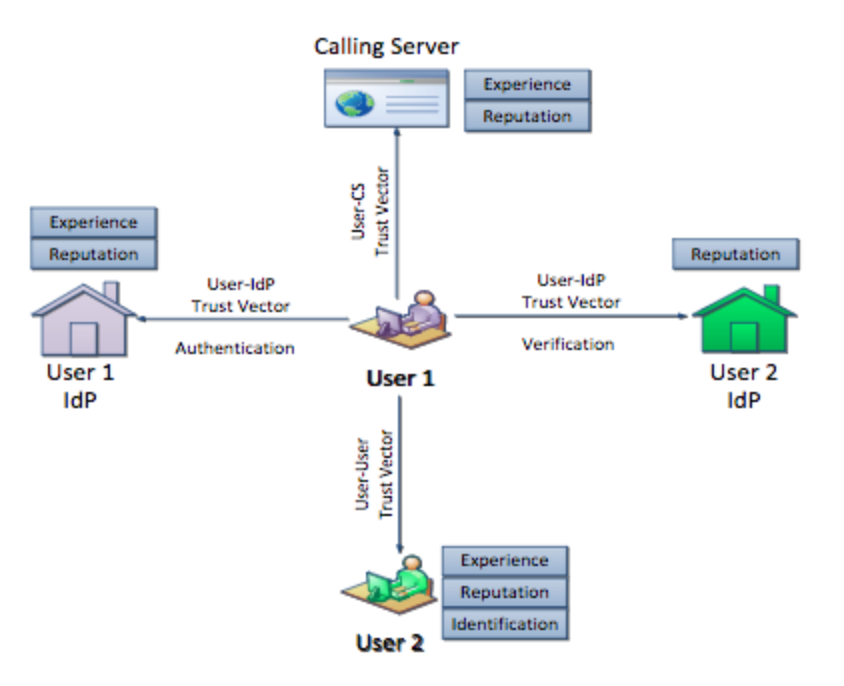
\includegraphics[scale=.8]{images/javed}
\end{center}
\caption{Javed \etal\cite{javed2016br2br} WebRTC trust model.}
\label{fig:javed}
\end{figure}

Copeland and Copeland proposed in 2016~\cite{copeland1question} a ``better than best effort'' architecture allowing communication services to select the appropriate network depending on selected profiles.
These profiles are built on balance between four considered criteria: QoS, Urgency, Security, and Affordability (QUSA).
Profiles and the associated network are selected based on the context of the communication. 
The context is derived from input from multiple sources, \eg calendar, social network, or location, with each source being attributed precision, accuracy, and confidence scores.
The overall architecture is summarised in Figure~\ref{fig:qusa}. 
The paper claims to have simulated 200 cases but point at the absence of real-world data.

\begin{figure}
\begin{center}
    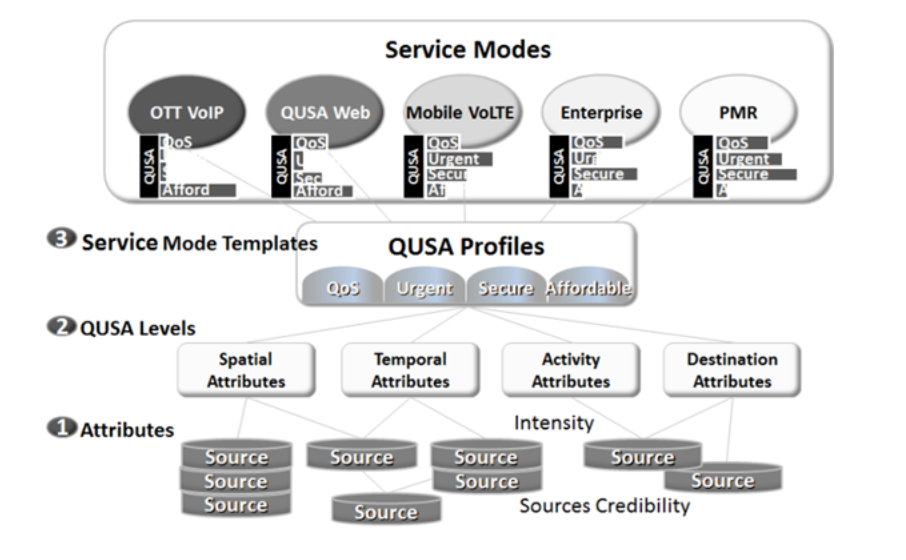
\includegraphics[scale=.8]{images/qusa}
\end{center}
\caption{Service Mode decision process based on context and QUSA profiles.}
\label{fig:qusa}
\end{figure}

\subsubsection{Social Threats (1)}
Following on their WebRTC trust model, Javed~\etal\cite{javed2017trustcall} propose a trust model evaluating trust in peers of a WebRTC communication in real-time.
In their model, a trust value is centrally computed by the communication service for each peer. 
This trust value is the weighted sum of an authenticity score, in fact a reputation, and a behavioural score based on talk time, incoming call numbers, and outgoing call numbers.
They simulate their approach and compare it to other trust models from the literature against some \gls{voip} social threats and trust model attacks.
Security considerations in this work are quite limited and only consider the authenticity of the other peer.
Furthermore, this authenticity of a peer is actually a reputation score rather than a measure of actual authentication.

In 2015, Vapen et al.~\cite{DBLP:conf/sec/VapenCMS15} studied the identity management landscape on the web\footnote{This paper is not part of our \gls{voip} security research collection.}. In their study, they classified the type of information shared by \gls{idp} to \gls{rp} in five classes: basic information, personal information, created content, friend's data, and a transversal action class.
They also defined semi-ordered risk types classes, build as conjunction of information shared classes. 
These classes range from R- to RA++ risk levels, A denoting action authorization.
In addition, their observations show that in practice \gls{rp} offer few choices of \gls{idp} to their users, with \SI{47}{\percent} offering only one \gls{idp}, and \SI{19}{\percent} offering four or more \gls{idp}. 
This situation profits to a few \gls{idp} trusting the top ranks, with Facebook as the number one, followed by Google and Twitter.

\subsubsection{Middleboxes (2)}
Johnston \etal\cite{johnston2013taking} look at the issues of WebRTC communication services in enterprise networks, \ie the traversal of enterprise firewalls for WebRTC session negotiated over \gls{https}.
They first present an overview of the issue and identify that current approaches for session border control and enterprise policies are not applicable to WebRTC.
The reason is that contrary to traditional \gls{voip} application using \gls{sip}, WebRTC applications may not expose sessions information to firewalls.
Several possible solutions are then described and discussed.
Other issues, not related to security, are also discussed such as the interoperation of WebRTC technologies with existing \gls{voip} infrastructures.

Singh \etal\cite{singh2015enterprise} implemented a Google Chrome extension to apply enterprise policies to WebRTC calls without help from underlying web application.
The extension overloads the WebRTC \gls{api} to intercept calls, it can then inserts user's enterprise identity in signalling messages.
Rather than implementing an \gls{idp} offering an \gls{idp} Proxy, the extension relies on an enterprise public key infrastructure to sign and verify signalling message.
The extension also forces the use of an enterprise media relay, \ie a modified \gls{turn} server responsible for applying enterprise's policies.

%\centering
\begin{table*}
\begin{tabular}{{@{}rlllllll@{}}}%\toprule\toprule
  &\textbf{Category / Title} & \textbf{Year} &\rotatebox{90}{\textbf{Security}} & \rotatebox{90}{\textbf{Trust}}& \rotatebox{90}{\textbf{Privacy}}& \rotatebox{90}{\textbf{Negotiation}}& \rotatebox{90}{\textbf{\gls{idp} Proxy}}\\\midrule

&\textbf{Social Threats}\\
\small{\cite{javed2017trustcall}}&\pbox{11cm}{\small{\textit{TrustCall: A Trust Computation Model for Web Conversational Services}}} & 2017 & & $\checkmark$ & & &  $\checkmark$ \\
\small{\cite{DBLP:conf/sec/VapenCMS15}}&\pbox{11cm}{\small{\textit{Information Sharing and User Privacy in the Third-Party Identity Management
               Landscape}}} & 2015 & & & $\checkmark$ \\
\midrule

&\textbf{Traffic Attacks}\\
\small{\cite{di2015decision}}&\pbox{11cm}{\small{\textit{A Decision Theory Based Tool for Detection of Encrypted WebRTC Traffic}}} & 2015 &  $\checkmark$ \\
\small{\cite{mauro_revealing_2017}}&\pbox{11cm}{\small{\textit{Revealing Encrypted WebRTC Traffic via Machine Learning Tools}}} & 2015 &  $\checkmark$ \\ 
\midrule

&\textbf{Overviews and Surveys}\\
\small{\cite{jennings2013real}}&\pbox{11cm}{\small{\textit{Real-time Communications for the Web}~}} & 2013 & $\checkmark$  & & & &  $\checkmark$\\ 
\small{\cite{barnes2014browser}}&\pbox{11cm}{\small{\textit{Browser-to-Browser Security Assurances for WebRTC}}} & 2014 & $\checkmark$ & & & &  $\checkmark$\\ 
\small{\cite{loreto_real-time_2012}}&\pbox{11cm}{\small{\textit{Real-Time Communications in the Web: Issue, Achievements, and Ongoing Standardization Efforts}}} & 2012 & $\checkmark$ \\ 
\small{\cite{loreto_how_2017}}&\pbox{11cm}{\small{\textit{How Far Are We from WebRTC-1.0?}}} & 2017 & $\checkmark$  & & & &  $\checkmark$\\ 
\small{\cite{rahaman2015survey}}&\pbox{11cm}{\small{\textit{A Survey on Real-Time Communication for Web}}} & 2015 & $\checkmark$  & & & &  $\checkmark$\\ 
\small{\cite{amirante2013seamless}}&\pbox{11cm}{\small{\textit{On the Seamless Interaction Between WebRTC Browsers and SIP-based Conferencing Systems}}} & 2013 & $\checkmark$ \\ 
\small{\cite{de2013web}}&\pbox{11cm}{\small{\textit{D.1.1 Web-platform security guide }}}  & 2013 & \checkmark \\
\small{\cite{bos2014case}}&\pbox{11cm}{\small{\textit{D1.2 Case Study: Security Assessment of WebRTC }}}  & 2014 & \checkmark \\
\midrule

&\textbf{Field Studies and System/Protocol Analysis}\\
\small{\cite{reiter2017webrtc}}&\pbox{11cm}{\small{\textit{WebRTC: Your Privacy Is at Risk}}} & 2017 & $\checkmark$ & & $\checkmark$ & &  $\checkmark$  \\
\small{\cite{al2017one}}&\pbox{11cm}{\small{\textit{One Leak Will Sink a Ship: WebRTC IP Address Leaks}}} & 2017 & & & $\checkmark$ \\
\midrule

&\textbf{Authentication Protocols}\\
\small{\cite{de2016ensuring}}&\pbox{11cm}{\small{\textit{Ensuring Endpoint Authenticity in WebRTC Peer-to-Peer Communication}}} & 2016 & $\checkmark$ & & & R & $\checkmark$\\
\midrule

&\textbf{Architectures}\\
\small{\cite{muranyi2013identity}}&\pbox{11cm}{\small{\textit{Identity Management in WebRTC Domains}}} & 2013 & & $\checkmark$ \\
\small{\cite{li2014calling}}&\pbox{11cm}{\small{\textit{Who Is Calling Which Page on the Web?}}} & 2014 & & $\checkmark$ & & &  $\checkmark$\\
\small{\cite{beltran2014user}}&\pbox{11cm}{\small{\textit{User Identity for WebRTC Services: A matter of trust}}} & 2014 & & $\checkmark$& $\checkmark$ \\
\small{\cite{beltran2015unified}}&\pbox{11cm}{\small{\textit{Unified Communications as a Service and WebRTC: an Identity-Centric Perspective}}} & 2015 & & $\checkmark$ & & &  $\checkmark$ \\
\small{\cite{beltran2015identity}}&\pbox{11cm}{\small{\textit{Identity Management for Web Business Communications}}} & 2015 & & $\checkmark$ & & & $\checkmark$\\
\small{\cite{javed2016browser}}&\pbox{11cm}{\small{\textit{Browser-to-Browser authentication and trust relationships for WebRTC}}} & 2016 & & $\checkmark$ & $\checkmark$ & &  $\checkmark$\\
\small{\cite{javed2016br2br}}&\pbox{11cm}{\small{\textit{Br2Br: a Vector-Based Trust Framework for WebRTC Calling Services}}} & 2016 & L  & $\checkmark$ & & &  $\checkmark$\\
\small{\cite{copeland1question}}&\pbox{11cm}{\small{\textit{A Question of Quality - VoIP, WebRTC or VoLTE?}}} & 2016 & & & & $\checkmark$ &$\checkmark$ \\
\midrule

&\textbf{Middleboxes}\\
\small{\cite{johnston2013taking}}&\pbox{11cm}{\small{\textit{Taking on WebRTC in an Enterprise}}} & 2013 & & P\\
\small{\cite{singh2015enterprise}}&\pbox{11cm}{\small{\textit{Enterprise WebRTC Powered by Browser Extensions}}} & 2015 &  & P & & & L\\

  \bottomrule
  \hline
\end{tabular}
\caption[Reviewed WebRTC Papers]{List of reviewed WebRTC papers. Checkmarks indicate whether the papers look or address the issues of security, trust model, privacy, security parameters negotiation, and the WebRTC identity architecture. The letters stand for L: \textit{limited}, R: \textit{recommends}, and P: \textit{policy trust}.}
\label{tab:SOTAobservations}
\end{table*}

\subsection{Observations}
We now compare the surveyed state of the art on WebRTC security to our research questions.
These observations allow us to narrow the focus of our contributions presented in later chapters.

Threats against user's security in the context of real-time multimedia communications and mechanisms to protect against these have been well-studied.
WebRTC has been built on this foundation, and the state of the art on \gls{voip} security research continued to develop since then.
As WebRTC is not a full-stack solution, we observe that researches on WebRTC and on WebRTC security mainly focus on security at the endpoint, including privacy risks for the users, and the issues of WebRTC deployment in enterprises.
One novelty introduced by the WebRTC security architecture is the integration of third-party \gls{idp} into the communication setup through the \gls{idp} Proxy mechanism.
This specification attracted a lot of interest from the community: as presented in Table~\ref{tab:SOTAobservations} we observe that out of 22 WebRTC security papers, a total of 13 papers reference the WebRTC identity architecture.
However, the security and privacy of this specification are only studied from a theoretical point of view~\cite{de2016ensuring}.
In particular, while WebRTC is intended to be interoperable with any \gls{sso} protocol, cross-implementation issues between the \gls{sso} protocol and WebRTC are rarely considered~\cite{li2014calling,de2016ensuring}.
The specification itself only sketches a short example using OAuth in annexe A~\cite{I-D.ietf-rtcweb-security-arch}. 
Additionally, other works study the privacy implications of the identity architecture but only consider the privacy threats posed by a malicious signalling server against user identity.
Consideration for this type of threats is already present in the WebRTC security architecture draft~\cite{I-D.ietf-rtcweb-security-arch}.
However, we do not observe research considering the privacy of the communication against the identity provider itself.

Besides understanding the threats faced by WebRTC users, we also want to act on a WebRTC session to raise the trust and security level.
Some surveyed work propose to negotiate the configuration of a WebRTC or \gls{voip} communication setup in order to achieve a given security level.
The solution of Copeland and Copeland~\cite{copeland1question} focus on selecting an appropriate underlying network, \ie at the network access layer, which does not allow to manage upper layer parameters.
Alia~\etal\cite{alia2010putting} propose an interesting model for balancing security and \gls{qos}.
However, their utility function is not convincing.
While an additive approach is coherent for modelling performance overheads, it does not achieve to model the dependent nature of security parameters.
For instance, a weak integrity on the signal path may have an important impact on confidentiality of the media path.

Increasing privacy, for instance to mitigate \gls{ice} \gls{ip} address leaks~\cite{al2017one}, mostly relies on permanent configuration options such as the selected \gls{os} or browser parameters.
Choosing proper actors to participate in the communication setup may also be a way to increase privacy, either because they implement privacy-preserving protocols or because they are trusted to not compromise user's privacy.
Regarding this last point, we note that De~Groef~\etal\cite{de2016ensuring} recommend that browsers allow users to select an \gls{idp} of their choice, \ie trusted, to participate in WebRTC sessions set up.

We want a model representing both security and trust to help users in the configuration and negotiation of WebRTC security parameters.
A lot of work has been conducted on modelling reputational-trust in WebRTC~\cite{beltran2014user,beltran2015unified,beltran2015identity,javed2016browser,javed2017trustcall}.
However, these papers generally do not consider the security of the session and the strength of security parameters in their models.
At most, only the user authentication strength is taken into account~\cite{javed2016br2br}.
Alternatively, some researchers~\cite{johnston2013taking,singh2015enterprise} consider trust policies with respect to WebRTC security.
However, they focus on applying enterprise policies and do not propose a complete model of WebRTC security.

\clearpage
\invisiblesection{Summary}
\label{sec:sotaSummary}
%\vspace*{3cm}

\blockmargin%
%\hspace{-\marginparwidth}\hspace{-\marginparsep}
\makebox[\overflowingheadlen][l]{
\begin{minipage}{\overflowingheadlen}

\begin{mdframed}[style=SOTAFrame,frametitle={\ref{sec:sotaSummary}~Summary}]

We conducted a research survey on \gls{voip} and WebRTC security research.
In total, we classified 208 research papers of which 23 were actually addressing WebRTC security. 
We then reported on the researches conducted in these 23 WebRTC security paper.

\medskip

Firstly, we observe that the WebRTC identity architecture attracted a lot of interest from the community.
However, we note that the security and privacy of the specification are only studied from a theoretical point of view~\cite{de2016ensuring}. 
In particular, the cross-implementation issues between \gls{sso} protocol and WebRTC are rarely considered~\cite{li2014calling,de2016ensuring}. 
The specification itself only sketches an implementation with the OAuth protocol in its annexe~\cite{I-D.ietf-rtcweb-security-arch}. 
We neither observe research considering the \gls{idp} as a possible attacker of the user's privacy.
In order to remedy to this issue, we intend to base our analysis of the WebRTC security and identity architecture on an actual implementation of \gls{sso} protocols in the context of a WebRTC service.

\medskip

Secondly, one of our research objectives is to build a model representing the trust and security of a WebRTC session and capable of returning a single metric.
In our survey, however, we do not observe research combining elements of trust and security models.
At best, one of the trust model uses limited security parameters~\cite{javed2016br2br} which confirms that combining trust and security for \gls{voip} is a novel approach.
Existing researchs work on the dynamic configuration of \gls{voip} services, but also uses a simplistic security model~\cite{alia2010putting}.
Nevertheless, other researchers recommend that users be given more control over which \gls{idp} they use in \gls{voip}~\cite{de2016ensuring} and more broadly on the Web~\cite{Sun2011}.
As we want to give them more control over the trust and security of their WebRTC session, we will focus on allowing users to negotiate WebRTC identity parameters. 

\end{mdframed}

\end{minipage}
}
\unblockmargin





%      \newgeometry{
%            left=2.2cm,
%            right=2.2cm,
%            top=2.2cm,
%            bottom=3.5cm,
%            ignoremp}
%      %\printbibliography
%      
%      \printbibliography[title={WebRTC Security State of the Art},keyword=sota]
%      
%      \clearpage
%      
%      
%    \restoregeometry
